\documentclass[a4paper,12pt]{report}
\usepackage[utf8]{inputenc}
\usepackage[T1]{fontenc}
\usepackage[italian]{babel}
\usepackage{listings}
\usepackage{graphicx}

\lstset{
    basicstyle=\ttfamily,
    columns=fullflexible,
    frame=single,
    breaklines=true,
    postbreak=\mbox{{$\hookrightarrow$}\space}
}

\makeatother


\title{\textbf{Relazione progetto} \break Traccia 3 - ``progetto''}
\author{Montali Giacomo - 0000925283 \\ Savini Edoardo - 0000921057}
\date{Giugno-Luglio 2021}

\begin{document}
	
\maketitle

\chapter{Introduzione}
Il progetto implementa un'architettura client-server per il supporto di un gioco multiplayer testuale in rete locale. Realizzato in Python 3, sfrutta un protocollo realizzato in maniera che sia facilmente scalabile e mantenibile per la comunicazione, permettendo in un futuro di aggiungere nuove funzioni senza fatica.
			
\chapter{Descrizione}
Partendo dall'idea di base del chat game abbiamo deciso di sviluppare un gioco sulla falsariga di \emph{Chi vuol essere milionario?} nel quale i giocatori si sfideranno con delle domande, che forniranno loro dei punti in base alla risposta data, il tutto accompagnato da una chat che permetterà loro di comunicare.

Inoltre nella stanza di gioco sarà presente un riquadro contenente la classifica in tempo reale. 

Le domande alle quali i giocatori dovranno rispondere avranno tre risposte ma solo una di queste sarà corretta. Per complicare il tutto, è stato inserito un timer, allo scadere del quale si passerà alla prossima domanda.

Prima dell'avvio della partita però, sarà richiesto al client di selezionare il proprio username e di connettersi al server che hosterà il gioco.
			
Il gioco prevede massimo dieci giocatori ma è facilmente modificabile (e aggirabile) nel codice questo limite fino ad arrivare al limite della macchina su cui viene eseguito.
			
\section{Scelte effettuate}

La prima scelta che abbiamo effettuato è stata quella del protocollo: il client e il server si scambiano messaggi JSON (linguaggio adatto all'interscambio dei dati con il quale abbiamo creato le nostre strutture, successivamente descritte dettagliatamente) che terminano con il carattere nullo (il primo della lista tabella ASCII con codice 0).

La scelta di far terminare tutti i messaggi con il carattere nullo è stata effettuata per permettere una facile ricezione ed elaborazione degli stessi man mano che i byte vengono estratti dal buffer.

L'interfaccia grafica è stata realizzata sulla falsariga di quanto già visto in tutti i giochi televisivi con delle domande.

\chapter{Dettagli implementativi}
	
\section{Strutture utilizzate}

Tutte le strutture dati hanno in comune la proprietà \emph{cmd} che permette di specificare quale comando è stato inviato, le altre proprietà dipendono da cosa si vuole inviare alla controparte.

Alla connessione viene aggiornata la leaderboard per far vedere quanti utenti sono connessi con il comando \emph{leaderboard}.

\begin{lstlisting}
{
    "cmd": "leaderboard",
    "leaderboard":[
        {
            "name": "Giacomo",
            "points": 200
        },
        {
            "name": "Edoardo",
            "points": 100
        }
    ]
}
\end{lstlisting}

Il primo comando che viene inviato dopo la pressione del bottone di avvio è \emph{start} che non prevede proprietà aggiuntive ed è solo un broadcast per ricevere dei dati da tutti i client.

\begin{lstlisting}
{
    "cmd": "start"
}
\end{lstlisting}
				
Tutti i client rispondono allo \emph{start} con il comando \emph{join} che invia anche il nome utente richiesto all'utente in fase di connessione.
				
\begin{lstlisting}
{
    "cmd": "join",
    "username": "Edoardo"
}
\end{lstlisting}


Il server invia contemporaneamente a tutti gli utenti (broadcast) il comando \emph{question} per aggiornare la domanda visualizzata. La struttura dati contiene una proprietà \emph{time} che indica i secondi a disposizione per rispondere.

\begin{lstlisting}
{
    "cmd": "question",
    "question": "Di che colore e' il cavallo bianco di napoleone?",
    "answers": [
        "rosso",
        "viola",
        "arancione",
        "verde"
    ],
    "time": 60
}
\end{lstlisting}

Quando l'utente risponde ad una domanda il client invia il comando \emph{answer} con una proprietà che indica l'indice della risposta selezionata (partendo da zero).

\begin{lstlisting}
{
    "cmd": "answer",
    "answer": 2
}
\end{lstlisting}

Scaduto il tempo, il server invia un broadcast (comando \emph{correction}) con la correzione delle risposte:

\begin{lstlisting}
{
    "cmd": "correction",
    "answer": 0
}
\end{lstlisting}

Quando un utente scrive un messaggio in chat, il client invia al server il comando \emph{sendMsg}.

\begin{lstlisting}
{
    "cmd": "sendMsg",
    "msg": "Hello, World!"
}
\end{lstlisting}

Il server procede poi all'inoltro del messaggio a tutti i client connessi con il comando \emph{receiveMsg}:

\begin{lstlisting}
{
    "cmd": "receiveMsg",
    "msg": "Hello, World!",
    "sender": "Giacomo"
}
\end{lstlisting}
				
Al termine della partita il server invia il comando \emph{winner}:

\begin{lstlisting}
{
    "cmd": "winner",
    "username": "Edoardo"
}
\end{lstlisting}
				
\section{Thread utilizzati}
\begin{itemize}

\item Thread Receiver, situato nei client, gestisce i messaggi ricevuti dal server per poi eseguire le operazioni necessarie per l'aggiornamento del gioco.
								
\item Thread Timer, che permette al programma di impostare un limite di tempo per ogni domanda.
								
\item Il thread principale che gestisce la grafica.

\end{itemize}
				
\section{Librerie utilizzate}	

\begin{itemize}
    \item tkinter
    
	\item thread
	
	\item json
    
    \item time
	
	\item socket, AF\_INET, SOCK\_STREAM
\end{itemize}

\chapter{Alcuni screenshot}

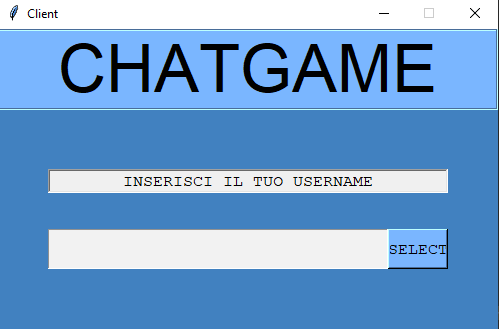
\includegraphics[width=\textwidth]{client_insertUsername.png}

\newpage

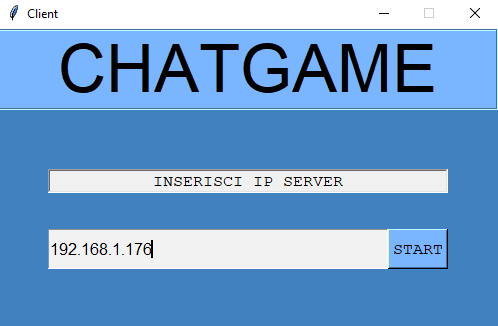
\includegraphics[width=\textwidth]{client_insertIP.png}

\newpage

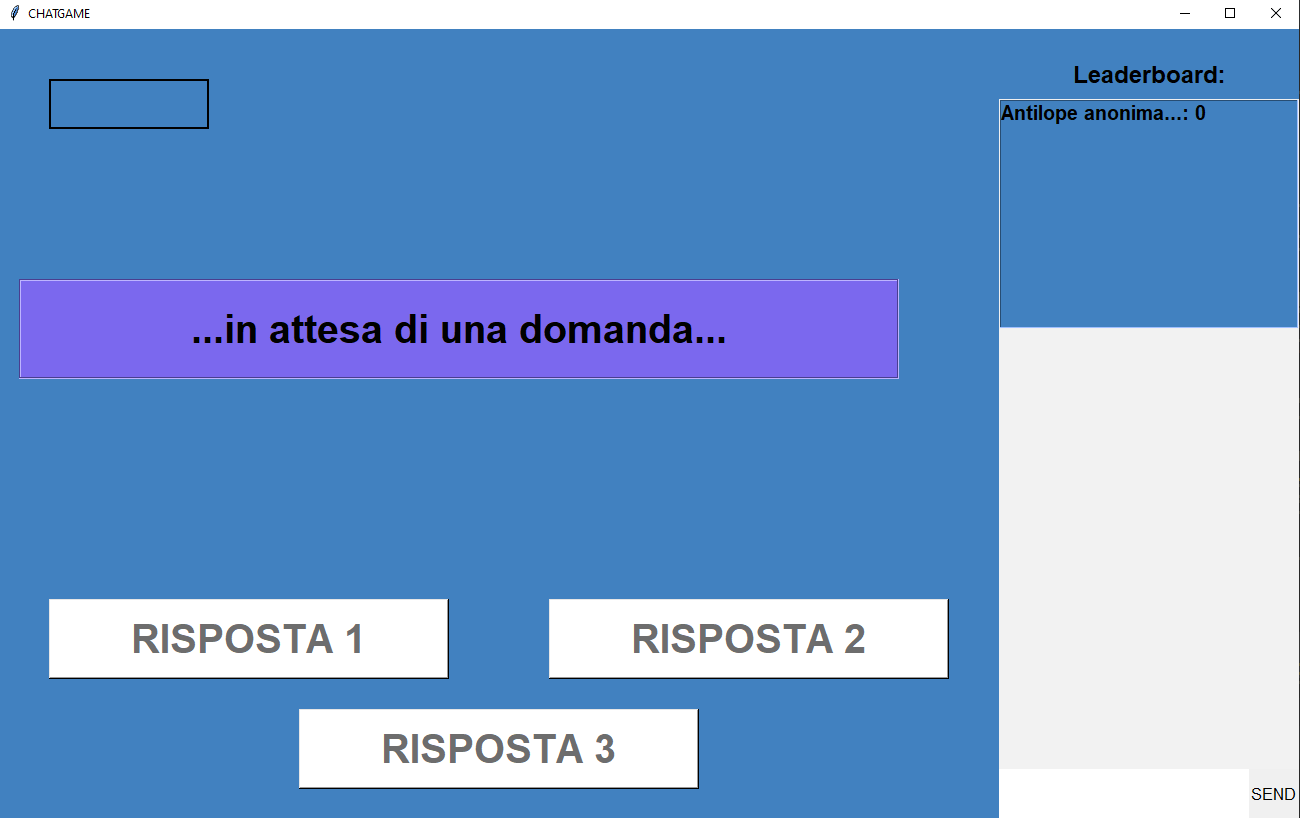
\includegraphics[width=\textwidth]{client_waitingGameStart.png}

\newpage

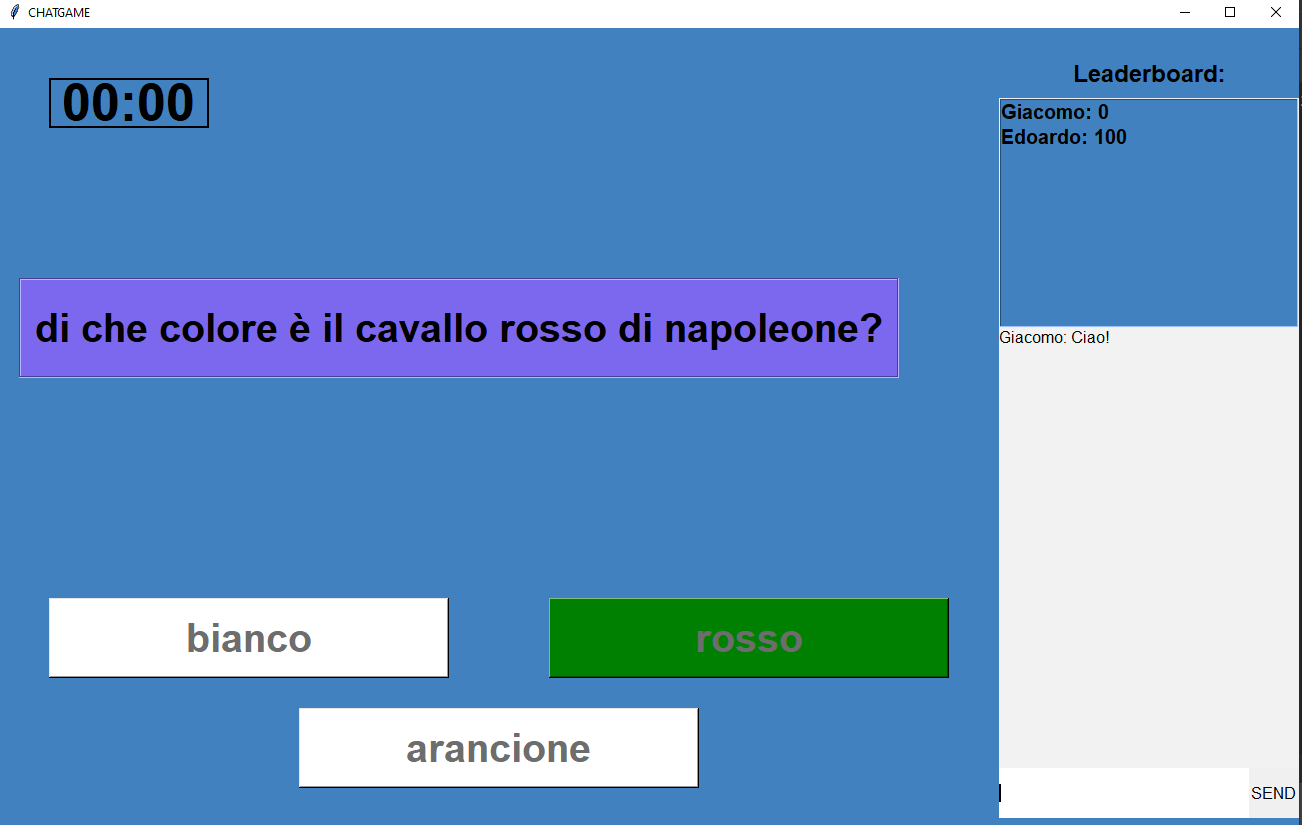
\includegraphics[width=\textwidth]{client.png}

\newpage

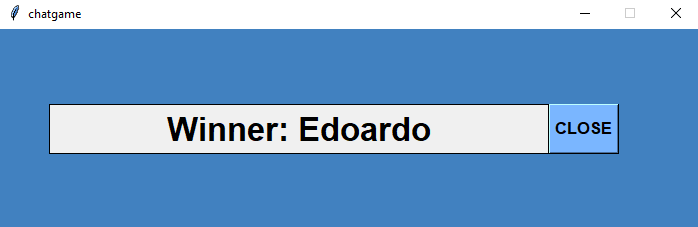
\includegraphics[width=\textwidth]{winner.png}

\newpage

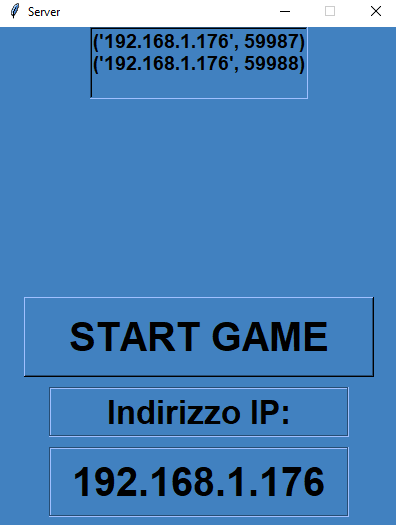
\includegraphics[width=\textwidth]{server.png}

\chapter{Avvio del server e del client}
Per avviare il server è sufficiente avviare \emph{server.py} mentre per il client \emph{client.py} (entrambi presenti nella root del repository).
	
\end{document}
